\documentclass[11pt]{article}
\usepackage[utf8]{inputenc}
\usepackage[brazil]{babel}
\usepackage{amsmath,amsfonts,amssymb,graphicx,mathtools}
\usepackage{hyperref}
\hypersetup{hidelinks}
\renewcommand{\baselinestretch}{1.1}
\usepackage{indentfirst}
\usepackage[table,xcdraw]{xcolor}
\usepackage{subcaption}
\usepackage{booktabs}
\usepackage{multirow}
\usepackage{geometry}
\usepackage{float}
\usepackage{titlesec}

\geometry{a4paper, left=1.5cm, right=1.5cm, top=1.6cm, bottom=1.6cm}
\setlength{\parindent}{1.25cm}
\setlength{\parskip}{0.08cm}
\captionsetup{font=small}

\setcounter{secnumdepth}{4}
\titleformat{\section}
{\normalfont\fontfamily{phv}\fontsize{12}{15}\selectfont\bfseries}{\thesection.}{1em}{}
\titleformat{\subsection}
{\normalfont\fontfamily{phv}\fontsize{12}{16}\selectfont\bfseries}{\thesubsection}{1em}{}
\renewcommand{\thesubsection}{\alph{subsection})}

\begin{document}

\begin{titlepage}
\begin{center}
{\Large \textbf{Universidade Federal de São Carlos}}\\
{\Large \textbf{Centro de Ciências Exatas e de Tecnologia}}\\
{\Large \textbf{Departamento de Estatística}}\\[1cm]


\includegraphics[scale=0.4]{ufscar-logo.png}\\[1cm]

{\Huge \textbf{Relatório do Projeto de Interpretabilidade de Modelos}}\\[0.8cm]
{\Huge \textbf{Grupo 5}}\\[1.5cm]

\begin{flushleft}
{\Large Arthur Pereira Gon \hfill RA: 811464}\\
{\Large Giovanni Roberti \hfill RA: 811676}\\
{\Large Igor Figueiredo Pereira da Silva \hfill RA: 791420}\\
{\Large Lucas Yukio Iyda \hfill RA: 813650}\\
{\Large Murilo Cassiavilani \hfill RA: 812067}
\end{flushleft}

\vspace{1.2cm}
{\Large Docente Helton Graziadei de Carvalho}

\vfill
{\Large São Carlos -- SP \quad 1º Semestre de 2026}\\[0.5cm]
\end{center}
\end{titlepage}

\section{Introdução}

Com o avanço do uso de modelos preditivos em diferentes áreas, tornou-se cada vez mais importante não apenas obter boas previsões, mas também compreender os fatores que levam o modelo a produzir determinado resultado. Em muitos problemas aplicados, avaliar apenas métricas de desempenho não é suficiente, pois modelos com resultados semelhantes podem utilizar as variáveis de formas diferentes. Dessa forma, a interpretabilidade passa a ter papel central na análise, permitindo investigar quais variáveis são mais relevantes, qual a direção de seus efeitos e se as relações identificadas fazem sentido no contexto do problema.

Nesse contexto, o presente projeto tem como objetivo investigar a interpretabilidade de modelos de regressão aplicados à predição de salários de jogadores da NBA. A análise busca compreender quais características individuais, estatísticas de desempenho e informações associadas ao contexto esportivo estão mais relacionadas ao salário anual dos jogadores na temporada 2022--2023.

Para isso, foram ajustados diferentes modelos de regressão, incluindo Regressão Linear Clássica, Regressão Ridge, Regressão Lasso, Random Forest e HistGradientBoosting. Essa escolha permite comparar modelos lineares e regularizados, cuja interpretação pode ser feita diretamente por meio dos coeficientes, com modelos baseados em árvores, que possuem maior flexibilidade para capturar relações não lineares e interações entre variáveis. Além da avaliação do desempenho preditivo, o trabalho aplica técnicas de interpretabilidade com o objetivo de responder a questões como: quais variáveis mais influenciam a predição dos salários? As relações identificadas fazem sentido no contexto da NBA? Os diferentes modelos apontam para conclusões semelhantes ou divergentes?

\section{Metodologia}

\subsection{Base de dados e definição do problema}

A base de dados utilizada contém informações de 467 jogadores da NBA referentes à temporada 2022--2023. Cada linha representa um jogador, descrito por características individuais, estatísticas de desempenho e informações da equipe. O objetivo é predizer o salário anual com base em estatísticas individuais, como pontos, assistências, rebotes e minutos em quadra, além de métricas avançadas de impacto esportivo.

Para manter correspondência com as colunas originais do dataset, as principais siglas são usadas ao longo do relatório: MP indica minutos por jogo; PTS, pontos; GP, jogos disputados; USG\%, taxa de uso ofensivo; PER, Player Efficiency Rating; BPM, Box Plus/Minus; VORP, valor sobre jogador de reposição; WS, Win Shares; AST, assistências; TOV, perdas de bola; STL, roubos; BLK, tocos; e PG, Point Guard.

\subsection{Análise exploratória dos dados}

A variável Salary, que representa o salário anual, apresenta média de US\$ 8,4 milhões e mediana de US\$ 3,7 milhões, indicando distribuição fortemente assimétrica à direita: poucos jogadores concentram contratos milionários. A idade média é 25,8 anos, com concentração entre 23 e 29 anos. As métricas de desempenho exibem elevada variabilidade, refletindo diferenças entre reservas, titulares e atletas de elite.

A Figura~\ref{fig:eda} resume os principais achados. A distribuição salarial confirma a assimetria positiva; o painel de correlações com salário mostra associação forte com PTS ($r = 0{,}73$), VORP ($r = 0{,}68$) e MP ($r = 0{,}64$). Também há multicolinearidade entre PER e BPM, com $r = 0{,}90$. Análises complementares indicam pico remuneratório entre 26 e 34 anos e maior salário médio entre jogadores PG.

\begin{figure}[H]
\centering
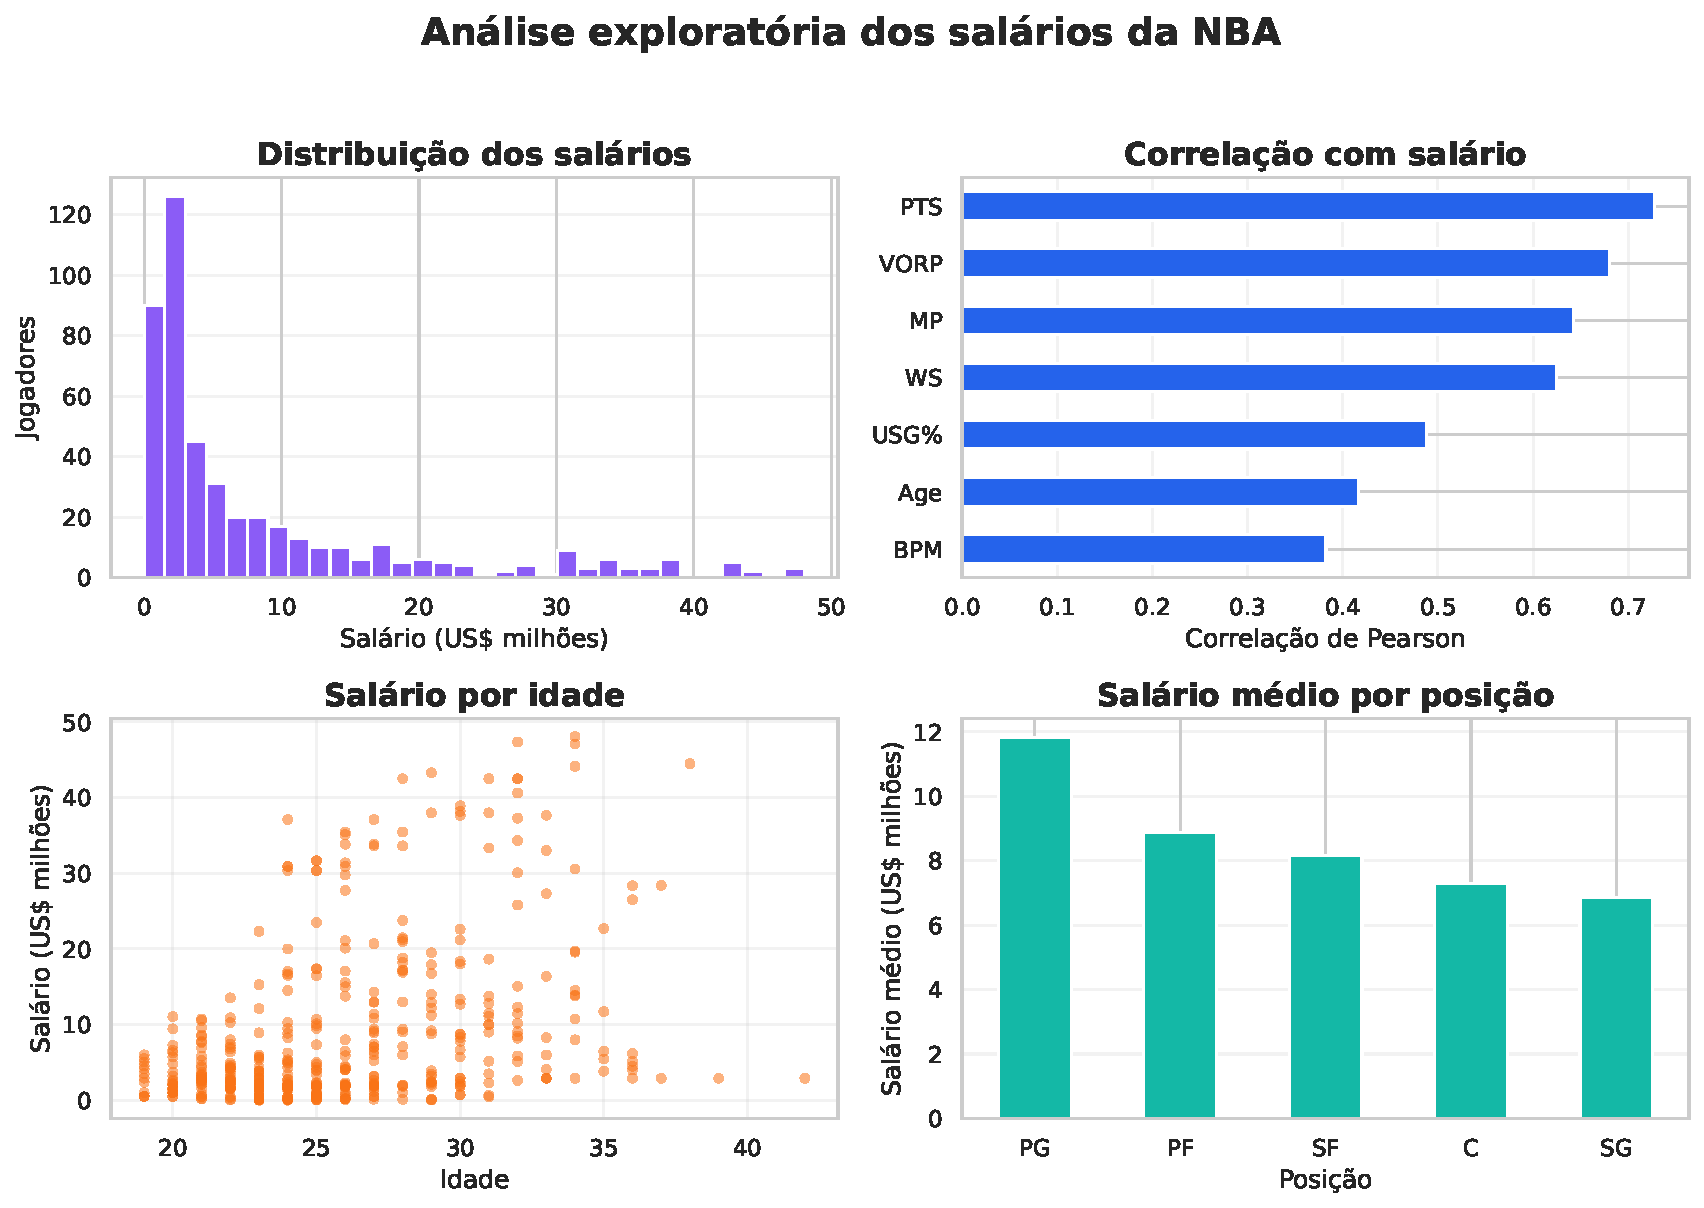
\includegraphics[width=0.98\textwidth]{eda_relatorio.pdf}
\caption{Análise exploratória dos salários: distribuição assimétrica, correlação com métricas de desempenho, efeito da idade e diferenças médias por posição.}
\label{fig:eda}
\end{figure}

\subsection{Pré-processamento}

Foram removidos 38 jogadores com salário inferior a US\$ 500.000 (contratos \textit{Two-Way}, de 10 dias ou proporcionais), reduzindo a base de 467 para 429 observações. Valores ausentes em percentuais de arremesso foram imputados pela mediana por posição, preservando diferenças estruturais entre armadores, alas e pivôs.

Aplicou-se transformação logarítmica em Salary, reduzindo a assimetria de 1,75 para aproximadamente 0,06 e melhorando a adequação dos modelos paramétricos. Criaram-se variáveis derivadas por jogo e por minuto, como Age\_sq, AST\_to\_TOV, STL\_BLK\_sum e Toxic\_Contract, além das categorias Rookie, Prime e Veteran. A centralização da idade reduziu o VIF de Age de 512 para 9,2. Variáveis redundantes, como TS\%, PER, WS, eFG\%, 3PAr e FTr, foram removidas; o VIF máximo final foi 13,8 para PTS\_per\_GP. O conjunto foi dividido em treino e teste (75/25), estratificado por posição ($n_{\text{teste}} = 108$).

\begin{table}[H]
\centering
\caption{VIF após o pré-processamento}
\label{tab:vif_depois}
\small
\begin{tabular}{lcc}
\toprule
\textbf{Variável} & \textbf{VIF} & \textbf{Status} \\
\midrule
PTS\_per\_GP & 13,8 & Marginalmente alto \\
MP & 11,1 & Marginalmente alto \\
STL\_BLK\_sum & 9,8 & Aceitável \\
Age & 9,2 & Aceitável \\
AST\_per\_min & 8,3 & Aceitável \\
BPM & 6,1 & Aceitável \\
\bottomrule
\end{tabular}
\end{table}

\subsection{Modelos ajustados e métricas}

Foram ajustados cinco modelos: OLS, Ridge ($L_2$), Lasso ($L_1$), Random Forest e HistGradientBoosting (HGB). Os modelos lineares permitem interpretação direta dos coeficientes; Ridge estabiliza estimativas sob multicolinearidade; Lasso realiza seleção de variáveis; Random Forest e HGB capturam não linearidades e interações. O desempenho foi avaliado por $R^2$, RMSE, MAE, MSLE e MAPE, na validação cruzada e no conjunto de teste (\textit{holdout}).

\subsection{Técnicas de interpretabilidade}

Nos modelos lineares, analisaram-se os coeficientes de OLS, Ridge e Lasso. No HGB, aplicaram-se importância por permutação (queda no $R^2$ ao embaralhar cada variável), valores SHAP (SHapley Additive exPlanations, contribuição marginal por observação) e Partial Dependence Plots (PDP), gráficos de dependência parcial que isolam o efeito médio de uma variável sobre a predição. O HGB foi escolhido como modelo principal para interpretação avançada por combinar menor MAPE (52,18\%) com capacidade de modelar relações não lineares, como o efeito parabólico da idade.

\subsection{Uso de ferramentas de Inteligência Artificial}

Ferramentas de Inteligência Artificial generativa foram utilizadas como apoio na revisão textual, melhoria da clareza da escrita acadêmica e organização de trechos de código. As decisões metodológicas, a escolha dos modelos, a análise dos resultados e as interpretações finais foram realizadas pelo grupo.

\section{Resultados e Discussão}

Foram avaliados cinco algoritmos de regressão. A Tabela~\ref{tab:resultados_modelos} apresenta o desempenho no conjunto de teste.

\begin{table}[H]
\centering
\caption{Desempenho dos modelos no conjunto de teste}
\label{tab:resultados_modelos}
\resizebox{\textwidth}{!}{
\begin{tabular}{lcccccc}
\toprule
\textbf{Modelo} & \textbf{$R^2$ Teste} & \textbf{RMSE (log)} & \textbf{MAE (log)} & \textbf{MSLE} & \textbf{MAE (USD)} & \textbf{MAPE} \\
\midrule
OLS & 0,5621 & 0,7569 & 0,5703 & 0,573 & 3.850.058 & 58,91\% \\
Ridge & 0,5878 & 0,7344 & 0,5474 & 0,539 & 3.721.480 & 55,34\% \\
Lasso & 0,5810 & 0,7405 & 0,5545 & 0,548 & 3.778.538 & 56,49\% \\
Random Forest & 0,5503 & 0,7671 & 0,5470 & 0,588 & 3.580.678 & 52,85\% \\
HistGradientBoosting & 0,5585 & 0,7600 & 0,5518 & 0,578 & 3.678.298 & 52,18\% \\
\bottomrule
\end{tabular}
}
\end{table}

O Ridge obteve o maior $R^2$ (0,5878), explicando cerca de 59\% da variabilidade salarial. O HGB e o Random Forest apresentaram os menores MAPE (52,18\% e 52,85\%). Todos os modelos ficaram na faixa $R^2 \in [0{,}55,\,0{,}59]$. Na validação cruzada, os modelos lineares foram mais estáveis (Tabela~\ref{tab:estabilidade}); o HGB equilibrou variância moderada com menor erro percentual.

\begin{table}[H]
\centering
\caption{Estabilidade na validação cruzada ($R^2$ CV std)}
\label{tab:estabilidade}
\small
\begin{tabular}{lcc}
\toprule
\textbf{Modelo} & \textbf{Std} & \textbf{Interpretação} \\
\midrule
OLS & 0,052 & Muito estável \\
Ridge & 0,063 & Estável \\
Lasso & 0,058 & Estável \\
Random Forest & 0,113 & Alta variância \\
HistGradientBoosting & 0,097 & Variância moderada \\
\bottomrule
\end{tabular}
\end{table}

\subsection{Interpretação dos modelos lineares}

Os coeficientes OLS representam efeitos marginais (\textit{ceteris paribus}). A Tabela~\ref{tab:coef_ols} destaca os principais preditores: MP (+0,74), Age (+0,57), categoria Rookie (+0,55) e USG\% (+0,21); Age\_sq ($-$0,16) confirma declínio pós-pico de carreira. Alguns coeficientes apresentam sinal aparentemente contraditório (PTS\_per\_GP $-$0,11; Position\_PG $-$0,12), reflexo de colinearidade residual entre métricas de desempenho. Por isso, devem ser interpretados com cautela, não como relações causais.

\begin{table}[H]
\centering
\caption{Principais coeficientes do modelo OLS}
\label{tab:coef_ols}
\small
\begin{tabular}{lcc}
\toprule
\textbf{Variável} & \textbf{Coeficiente} & \textbf{Interpretação} \\
\midrule
MP & +0,74 & Principal preditor salarial \\
Age & +0,57 & Idade aumenta salário até o pico \\
Experience\_Category\_Rookie & +0,55 & Efeito contratual rookie scale \\
USG\% & +0,21 & Participação ofensiva valorizada \\
Age\_sq & $-$0,16 & Declínio pós-pico de carreira \\
AST\_per\_min & +0,10 & Eficiência de passe \\
BPM & +0,10 & Impacto geral no jogo \\
\bottomrule
\end{tabular}
\end{table}

A comparação Ridge versus Lasso (Tabela~\ref{tab:ridge_lasso}) confirma robustez: MP (+0,56 / +0,69), Age (+0,41 / +0,48) e USG\% (+0,18 / +0,20) mantêm sinais consistentes. O Lasso foi mais agressivo na seleção, zerando variáveis menos relevantes.

\begin{table}[H]
\centering
\caption{Comparação entre coeficientes Ridge e Lasso}
\label{tab:ridge_lasso}
\small
\begin{tabular}{lcc}
\toprule
\textbf{Variável} & \textbf{Ridge} & \textbf{Lasso} \\
\midrule
MP & +0,56 & +0,69 \\
Age & +0,41 & +0,48 \\
Age\_sq & $-$0,06 & $-$0,09 \\
USG\% & +0,18 & +0,20 \\
Rookie & +0,21 & +0,33 \\
Veteran & +0,25 & +0,21 \\
\bottomrule
\end{tabular}
\end{table}

\subsection{Interpretação do HistGradientBoosting}

A interpretação do HistGradientBoosting foi organizada do comportamento global para a explicação local. Primeiro, avaliou-se quais variáveis sustentam o desempenho do modelo; depois, analisou-se a direção dos efeitos por SHAP; por fim, foi escolhido um jogador específico para mostrar como a predição é formada.

A importância por permutação confirma a dominância de MP (0,452) e Age (0,262). Embaralhar MP reduz o $R^2$ em cerca de 0,45 pontos no teste (aproximadamente 81\% do desempenho do modelo); juntas, MP e Age somam importância acumulada de 0,71, evidenciando que tempo em quadra e estágio da carreira concentram grande parte da informação salarial. PTS\_per\_GP (0,041) e USG\% (0,023) aparecem em um segundo nível, indicando que produtividade ofensiva importa, mas principalmente depois de controlar utilização e estágio da carreira.

O PDP mostra que o salário previsto cresce até aproximadamente 28--30 anos e depois declina gradualmente. O resumo SHAP acrescenta a direção dos efeitos: valores altos de MP deslocam a predição para cima, enquanto idades fora do pico tendem a reduzir o salário previsto. Para melhorar a leitura, as figuras SHAP mantêm apenas as variáveis de maior impacto e agregam o restante em ``Outras variáveis''.

\begin{figure}[H]
\centering
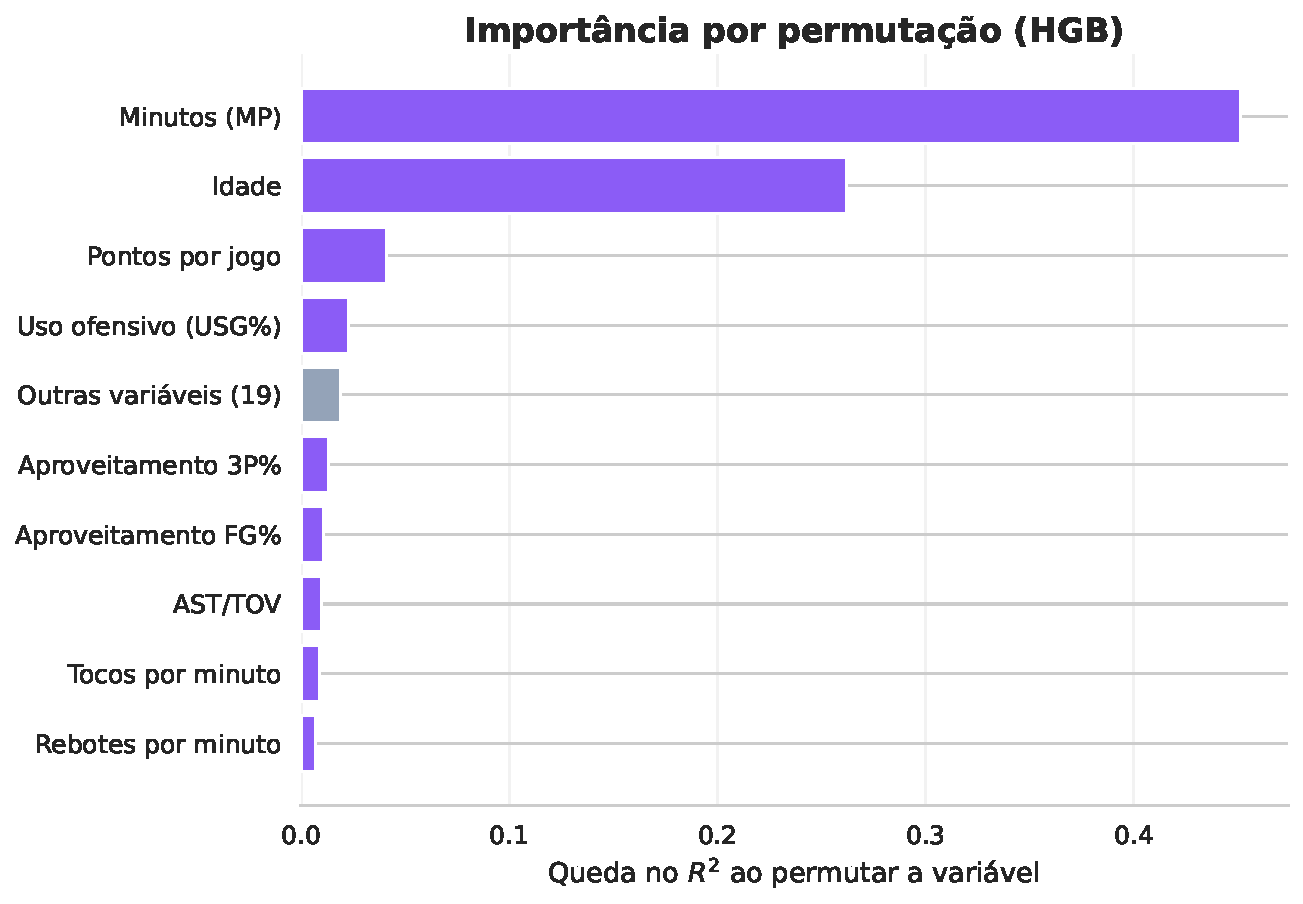
\includegraphics[width=0.82\textwidth]{importancia_relatorio.pdf}

\vspace{0.25cm}
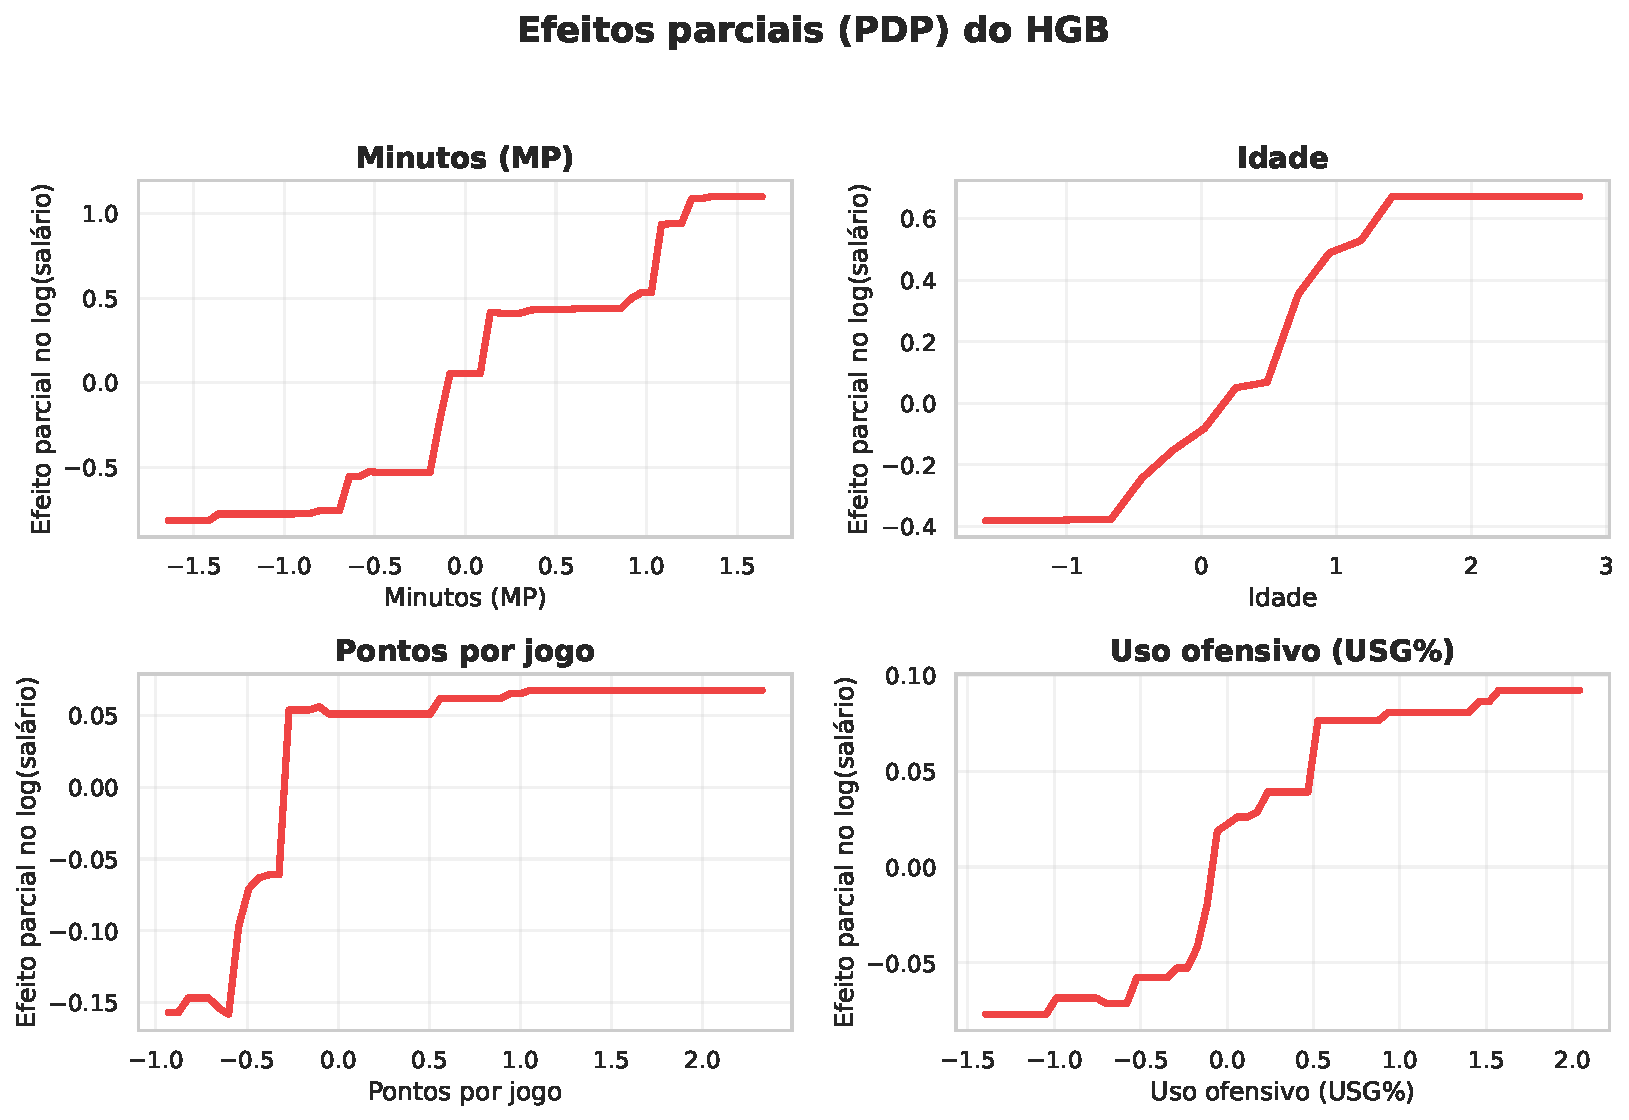
\includegraphics[width=0.99\textwidth]{pdp_relatorio.pdf}
\caption{Interpretação global do HistGradientBoosting: importância por permutação e efeitos parciais das quatro variáveis mais relevantes.}
\label{fig:interpretabilidade_hgb}
\end{figure}

\begin{figure}[H]
\centering
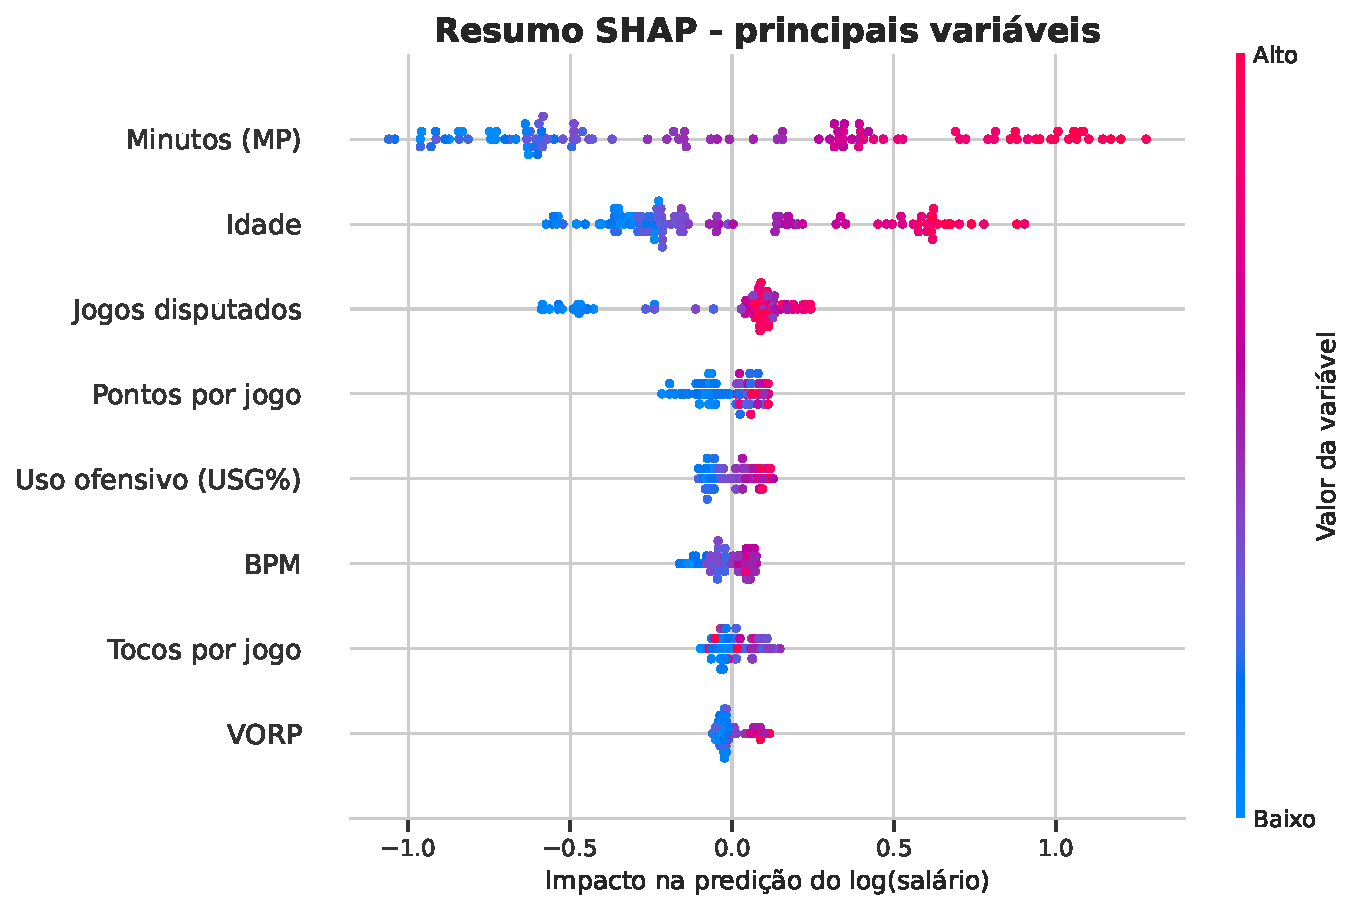
\includegraphics[width=0.98\textwidth]{shap_summary_relatorio.pdf}
\caption{Resumo SHAP do HistGradientBoosting com as principais variáveis. Cada ponto representa um jogador; a posição horizontal indica quanto a variável aumentou ou reduziu a predição.}
\label{fig:shap_hgb}
\end{figure}

\begin{figure}[H]
\centering
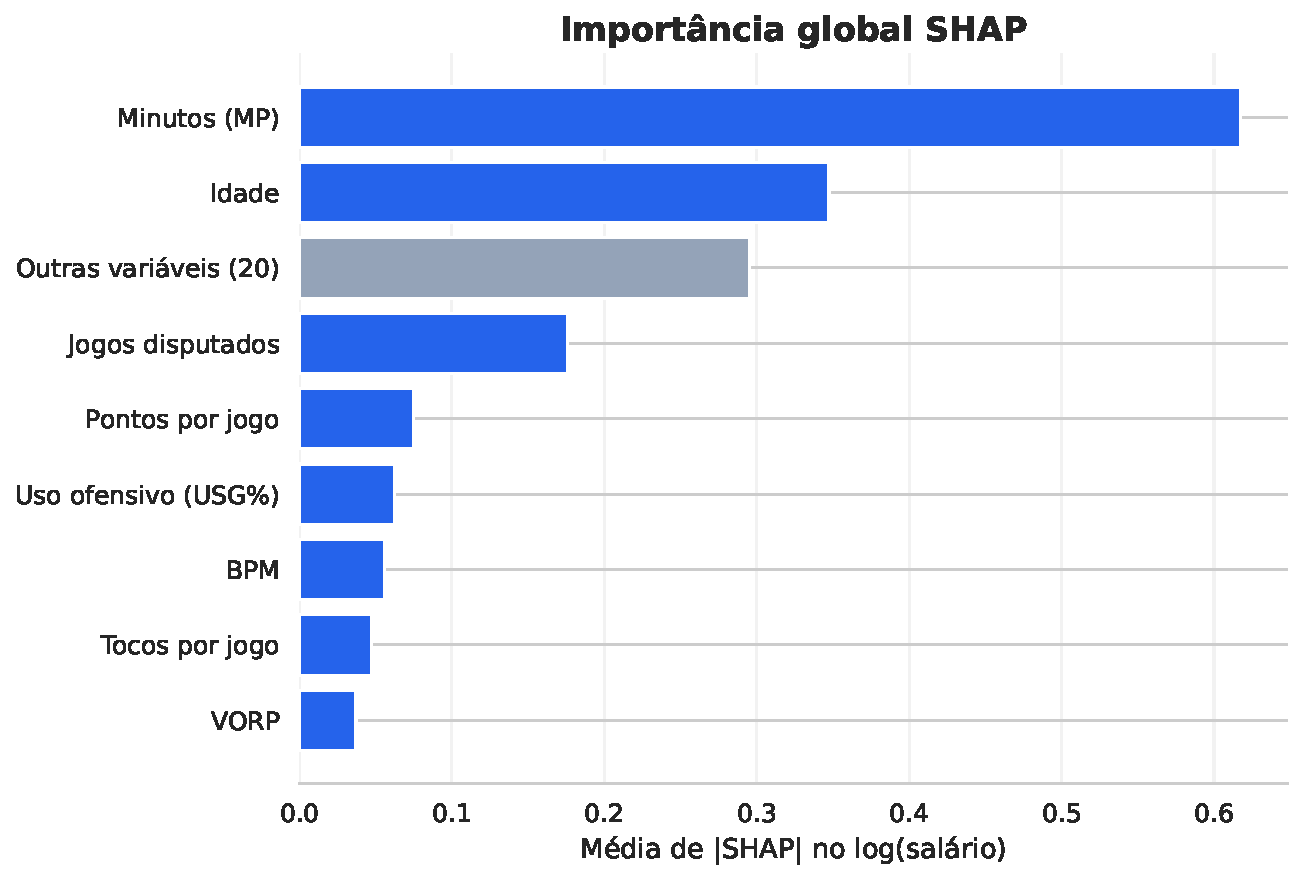
\includegraphics[width=0.76\textwidth]{shap_global_relatorio.pdf}
\caption{Importância global SHAP com ``Outras variáveis'' acumulado.}
\label{fig:shap_global_waterfall}
\end{figure}

Para a leitura local, escolheu-se Stephen Curry por ser um caso bem previsto: US\$ 46,3 milhões estimados contra US\$ 48,1 milhões observados.

\begin{figure}[H]
\centering
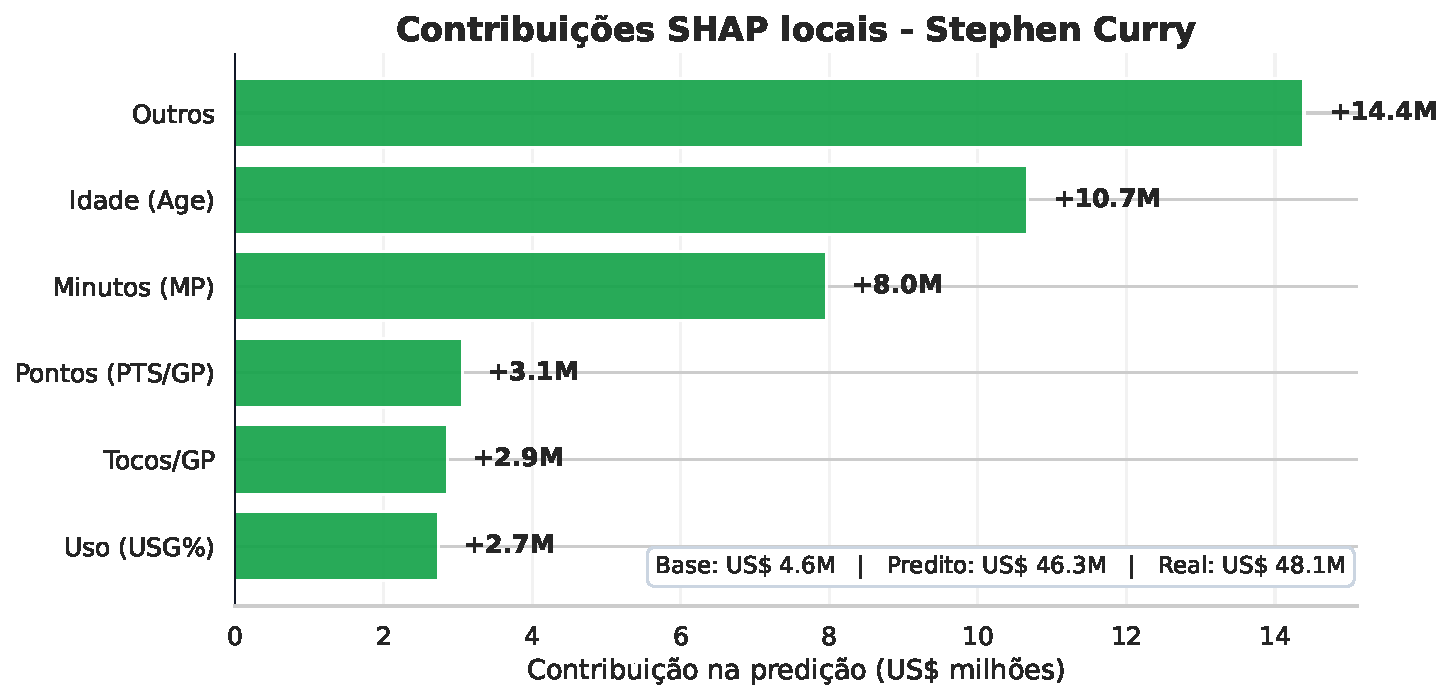
\includegraphics[width=0.86\textwidth]{shap_curry_contribuicoes_relatorio.pdf}
\caption{Contribuições SHAP locais para Stephen Curry, em milhões de dólares. O grupo ``Outras'' reúne contribuições menores que, individualmente, teriam baixa legibilidade.}
\label{fig:shap_curry_final}
\end{figure}

\subsection{Limitações e maiores erros}

A leitura local de Curry mostra um caso em que o modelo acerta bem um jogador de elite. Em contraste, a Tabela~\ref{tab:maiores_erros} apresenta os maiores erros no teste. Kemba Walker (erro de US\$ 32,5 milhões, 87\%) exemplifica contratos tóxicos: salário elevado por acordo anterior, com baixa participação recente. Casos como Russell Westbrook e Jonathan Isaac envolvem supermax antigo e lesões graves, fatores ausentes na base. O modelo captura bem a remuneração baseada em desempenho, mas não incorpora dinâmica contratual e mercadológica da NBA.

\begin{table}[H]
\centering
\caption{Maiores erros de previsão no conjunto de teste}
\label{tab:maiores_erros}
\small
\resizebox{\textwidth}{!}{
\begin{tabular}{lcccc}
\toprule
\textbf{Jogador} & \textbf{Real} & \textbf{Predito} & \textbf{Erro (USD)} & \textbf{Principal causa} \\
\midrule
Kemba Walker & 37,3M & 4,8M & 32,5M & Contrato tóxico \\
Myles Turner & 35,1M & 9,4M & 25,7M & Extensão contratual \\
Russell Westbrook & 47,1M & 28,9M & 18,2M & Supermax antigo \\
Shai Gilgeous-Alexander & 30,9M & 13,0M & 17,9M & Extensão jovem \\
Jonathan Isaac & 17,4M & 0,7M & 16,7M & Lesões graves \\
\bottomrule
\end{tabular}
}
\end{table}

\section{Conclusão}

O projeto mostrou que estatísticas de quadra explicam parcela relevante dos salários da NBA, mas não capturam integralmente fatores contratuais e mercadológicos. Os modelos tiveram desempenho semelhante ($R^2 \approx 0{,}55$--$0{,}59$), com maior $R^2$ no Ridge e menor MAPE no HGB. As técnicas de interpretabilidade convergiram para a mesma leitura: minutos jogados e idade são os principais determinantes salariais, seguidos por produtividade ofensiva. Casos extremos, como contratos antigos e jogadores lesionados, evidenciam as limitações da base, enquanto coeficientes, permutation importance, PDP e SHAP tornam as previsões mais transparentes.

\end{document}
